\documentclass[t,xcolor={usenames,dvipsnames}]{beamer}

\mode<presentation>
{
\usetheme{Frankfurt}%{Warsaw}
%\setbeamercovered{transparent}
%\setbeamercolor{background canvas}{bg=white}
}

% Delete these, if you do not want the table of contents to pop up at
% the beginning of each (sub)section:
%\AtBeginSubsection[]
%{
%  \begin{frame}<beamer>{Outline}
%    \tableofcontents[currentsection,currentsubsection]
%  \end{frame}
%}
%\AtBeginSection[]
%{
%  \begin{frame}<beamer>{Outline}
%    \tableofcontents[currentsection]
%  \end{frame}
%}

\usepackage[english]{babel}
\usepackage[latin1]{inputenc}
\usepackage{times}
\usepackage[T1]{fontenc}
\usepackage{verbatim}
\usepackage{url}
\usepackage{amsmath,amssymb}
\usepackage{comment}
\usepackage[overlay,absolute]{textpos}
\usepackage{hyperref}

% Author-date citations
\usepackage[authoryear,round]{natbib}
\let\cite=\citep  % default \cite such as {\LaTeX} authors are used to

% Where \includegraphics should look for figures
\graphicspath{{./figs/}{../group_talk_2011_11_29/figs/}}
\usepackage{epstopdf}
\DeclareGraphicsExtensions{.eps,.png,.jpg,.pdf}

% Shortcuts
\newcommand{\myhref}[2]{\href{#1}{\textcolor{Blue}{#2}}}
\newcommand{\myurl}[1]{\myhref{#1}{#1}}
\newcommand{\subitem}[1]{\begin{itemize}[<.->]\item #1 \end{itemize}}
\newcommand{\ghead}[1]{{\tiny #1\\}}
\newcommand{\doi}[1]{\myhref{http://dx.doi.org/#1}{doi:#1}}
\newcommand{\csym}[1]{\textcolor{Blue}{\texttt{#1}}}
\newcommand{\ud}{\mathrm{d}}
\newcommand{\dt}{\ud t}

%%%%%%%%%%%%%%%%%%%%%%%%%%%%%%%%%%%%%%%%%%%%%%%%%%%%%%%%%%%%%%%%%%%%%%
\title{Functional Curation}
\author{Jonathan Cooper}
\institute[University of Oxford]
{Computational Biology Group\\
 Department of Computer Science\\
 University of Oxford}
\date{February 7, 2014}

\begin{document}

\begin{frame}
% I'm going to talk about: why we developed functional curation, what it is,
% a few brief examples, and where we're hopefully heading.
\titlepage
\end{frame}

\begin{comment}
From Greg:
Looking forward to the workshop next week. There will be 12 of us, big enough to get a good idea about the scope of work and possibilities, but small enough that we can have an intensive discussion where needed. It is a multidisciplinary crowd from ecology and maths, to computer science and web development.

As discussed, could you talk about the following in 10 mins +5 for questions (or 15 and no questions :)
�       Dave - online repositories overview
�       Jon - Functional Curation overview
�       Gary - Functional Curation in action
The ecologists are a smart bunch, but more expert in statistics than mathematics and computer science. I'll do a brief introduction to tie things together.
\end{comment}

%%%%%%%%%%%%%%%%%%%%%%%%%%%%%%%%%%%%%%%%%%%%%%%%%%%%%%%%%%%%%%%%%%%%%%

%\begin{frame}{Outline}
%\setcounter{tocdepth}{1}
%\tableofcontents
%\end{frame}

%%%%%%%%%%%%%%%%%%%%%%%%%%%%%%%%%%%%%%%%%%%%%%%%%%%%%%%%%%%%%%%%%%%%%%
\section{Motivation}
\subsection*{Main}
%%%%%%%%%%%%%%%%%%%%%%%%%%%%%%%%%%%%%%%%%%%%%%%%%%%%%%%%%%%%%%%%%%%%%%

\begin{frame}{Modelling biology}
\begin{itemize}
\item A mathematical model encodes a quantitative hypothesis about a biological system
\item It can be used to make predictions about the response of the system to experiments
  \subitem{``If I make this intervention, I expect to see that change''}
\item Increasingly, models build on previously published models
  \begin{itemize}
  \item Compose models together to study larger system
    % examples: reaction networks, nephrons/kidneys, heart
  \item Extend or modify models to incorporate latest understanding, or look at effect of disease / drug / species / age / \ldots
  \end{itemize}
\end{itemize}
\end{frame}


\begin{frame}{Using models}
\begin{itemize}
\item As hypothesis encodings, models are developed \emph{for a specific purpose}
  \subitem{May not be appropriate for studying same system in different context}
\item How can we\ldots
  \begin{itemize}
  \item determine a model's functionality, i.e.\ its suitability or limitations for a new study?
  \item re-use a model in a different experimental context?
  \item compare hypotheses: different models' behaviours under the same experiment?
  \end{itemize}
\end{itemize}
\end{frame}


\begin{frame}{Models and experiments}
% Not so much the details that matter here, as the background to how we
% created our current approach.  Focus on type of model, and range of
% interventions possible.
\small
Suppose we have our mathematical model, e.g.\ Hund \& Rudy 2004:\\
\includegraphics[width=\textwidth]{hund_2004}\\
We want to perform various potentially complex interventions\ldots
\end{frame}


\begin{frame}{Experiment: $I_{\textrm{Ca}_L}$ voltage clamp}
\begin{center}
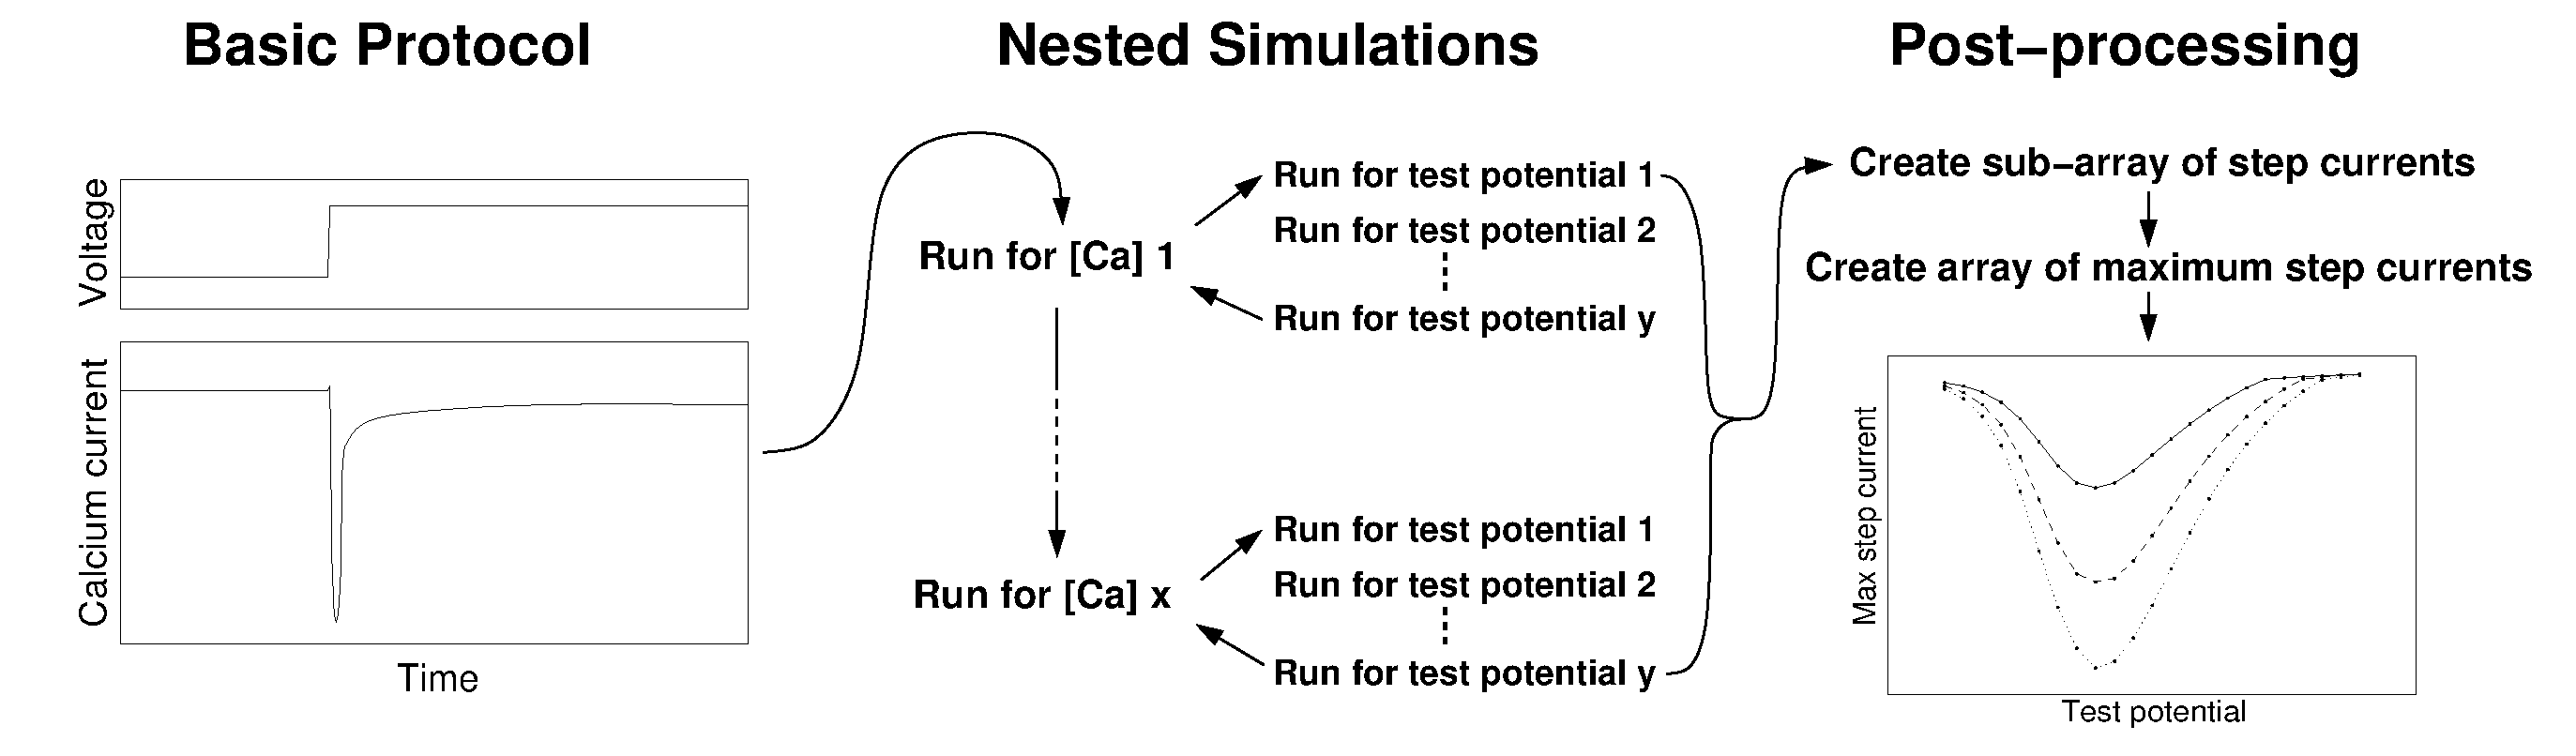
\includegraphics[width=\textwidth]{ICaLIntro}
\end{center}
\begin{itemize}
\item This experiment isolates a single ion channel in the cell membrane, and controls the external ion concentrations and voltage
\item Most of the model equations are thus either altered or irrelevant
\end{itemize}
\end{frame}


\begin{frame}{Experiment: S1-S2 restitution}
\begin{center}
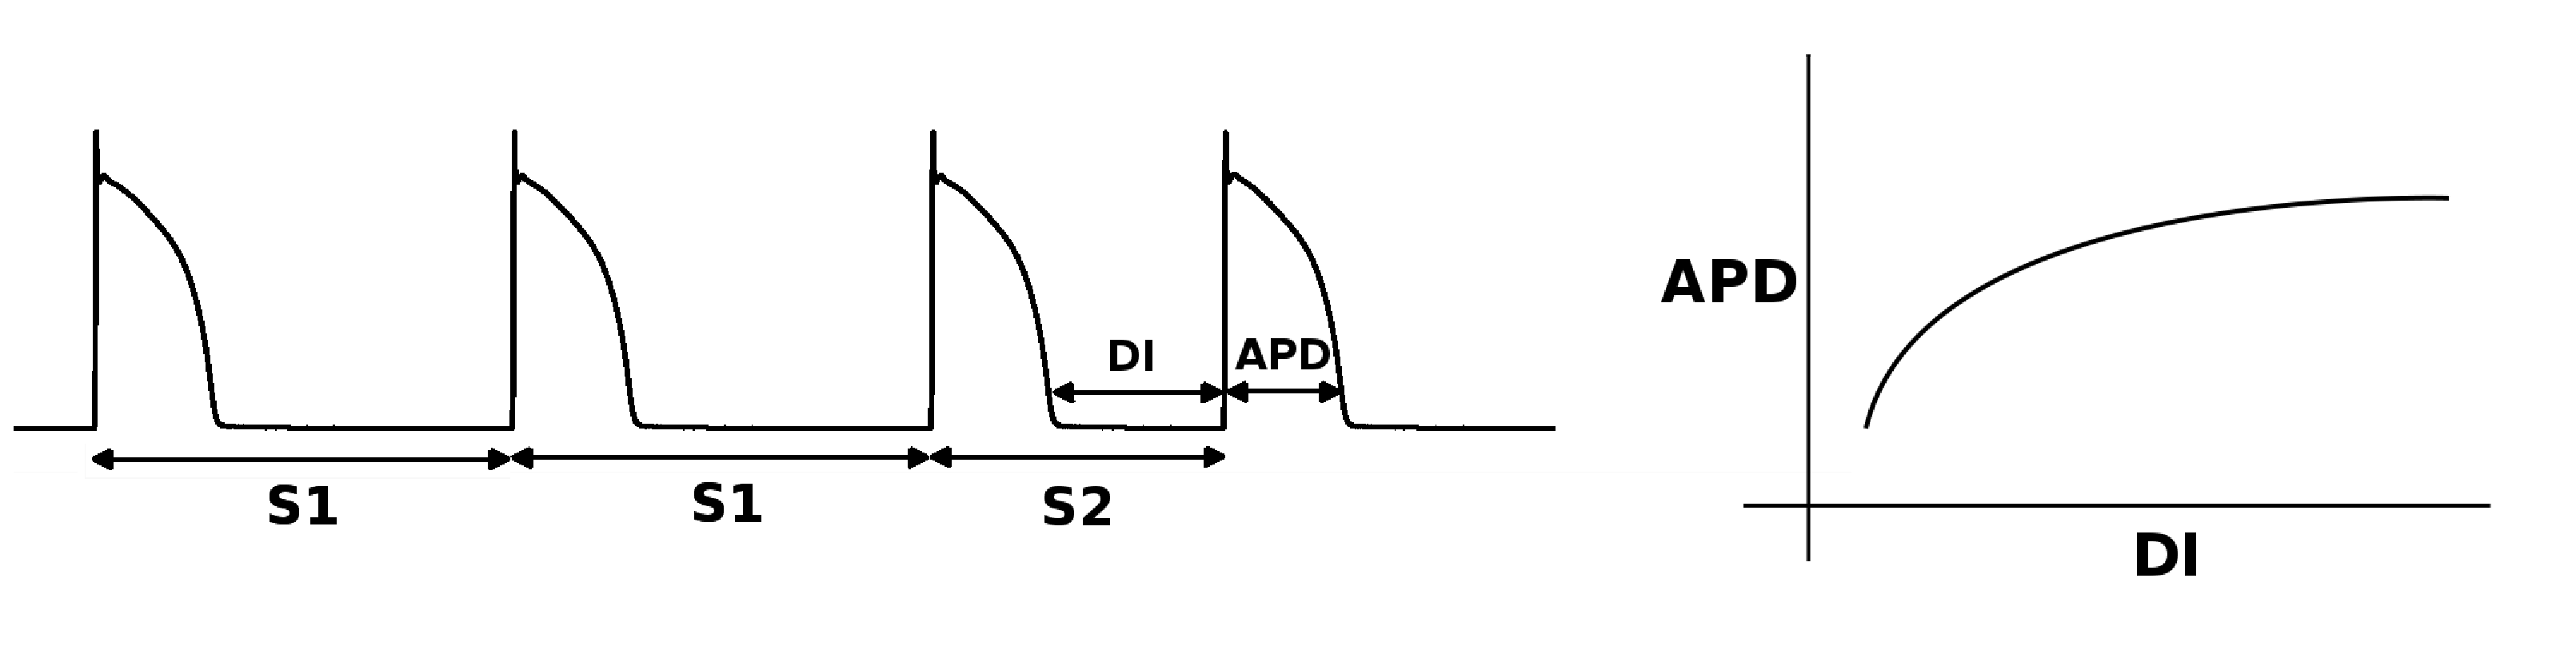
\includegraphics[width=\textwidth]{S1S2}
\end{center}
\begin{itemize}
\item Here it is the post-processing to compute the action potential durations (APDs) that is most complex
\end{itemize}
\end{frame}


%%%%%%%%%%%%%%%%%%%%%%%%%%%%%%%%%%%%%%%%%%%%%%%%%%%%%%%%%%%%%%%%%%%%%%
\section{Functional curation with virtual experiments}
\subsection*{Main}
%%%%%%%%%%%%%%%%%%%%%%%%%%%%%%%%%%%%%%%%%%%%%%%%%%%%%%%%%%%%%%%%%%%%%%

\begin{frame}{The essence}
\subitem{Separate \alert{model structure} and \alert{experimental scenario}}
\vspace{-.2cm}
\hspace{-1cm}\includegraphics[width=1.185\textwidth]{virtual_expts_schematic}
\vspace{-.31cm}
\begin{itemize}
\item Apply any \alert{virtual experiment} to any (relevant) model
\item One definitive version of each model / protocol
\item Automatically generate post-processed outputs, plots, etc.
\end{itemize}
\end{frame}


\begin{frame}{What goes in a protocol?}
\begin{itemize}
\item Definition of the interface with the model being experimented on
  \begin{itemize}
  \item Handle variations in modelling conventions: naming, encoding the biology in mathematics
  \item Units conversions
  \item Isolate relevant sub-model(s), using model inputs \& outputs of interest
  \end{itemize}
\item Definition of simulations to perform
\item Post-processing operations on simulation results
\item Description of what to plot
\vspace{.5cm}
\item Also language features facilitating building complex protocols, e.g.\ protocol inputs, outputs, and imports.
\end{itemize}
\end{frame}


%%%%%%%%%%%%%%%%%%%%%%%%%%%%%%%%%%%%%%%%%%%%%%%%%%%%%%%%%%%%%%%%%%%%%%
\section{Examples}
\subsection*{Main}
%%%%%%%%%%%%%%%%%%%%%%%%%%%%%%%%%%%%%%%%%%%%%%%%%%%%%%%%%%%%%%%%%%%%%%

\begin{frame}{Example: S1-S2 restitution on canine models}
\begin{columns}[T]
\begin{column}{.33\linewidth}
\begin{center}
\includegraphics[width=\textwidth]{sicouri_dog_ventricle_s1s2_curve}\\
\vspace{.1cm}
\includegraphics[width=\textwidth]{hund_rudy_2004_s1s2_curve}
\end{center}
\end{column}
\begin{column}{.33\linewidth}
\begin{center}
\includegraphics[width=\textwidth]{winslow_model_1999_s1s2_curve}\\
\vspace{.1cm}
\includegraphics[width=\textwidth]{livshitz_rudy_2007_s1s2_curve}
\end{center}
\end{column}
\begin{column}{.33\linewidth}
\begin{center}
\includegraphics[width=\textwidth]{fox_mcharg_gilmour_2002_s1s2_curve}\\
\vspace{.1cm}
\includegraphics[width=\textwidth]{decker_2009_s1s2_curve}
\end{center}
\end{column}
\end{columns}
\end{frame}


\begin{frame}{Example: $I_{\textrm{Ca}_L}$ voltage clamp}
\begin{columns}[T]
\begin{column}{.33\linewidth}
\begin{center}
\includegraphics[width=\textwidth]{sun_rat_ventricle_ICaL_IV_curve}\\
\vspace{.1cm}
\includegraphics[width=\textwidth]{fink_noble_giles_model_2008_ICaL_IV_curve}
\end{center}
\end{column}
\begin{column}{.33\linewidth}
\begin{center}
\includegraphics[width=\textwidth]{bondarenko_szigeti_bett_kim_rasmusson_2004_apical_ICaL_IV_curve}\\
\vspace{.1cm}
\includegraphics[width=\textwidth]{grandi_pasqualini_bers_2010_ss_ICaL_IV_curve}
\end{center}
\end{column}
\begin{column}{.33\linewidth}
\begin{center}
\includegraphics[width=\textwidth]{ten_tusscher_model_2006_epi_ICaL_IV_curve}\\
\vspace{.1cm}
\includegraphics[width=\textwidth]{corrias_purkinje_2011_ICaL_IV_curve}
\end{center}
\end{column}
\end{columns}
\end{frame}


\begin{frame}{Intestinal crypts}
% Main point here is that we're not just interested in cardiac: have started
% to look at how approach generalises to other domains, and want to know if
% SDM could be one of them
\begin{itemize}
\item Here a `model' is a \alert{simulation} of a collection of interacting cells, not just equations
  \subitem{Implemented using the cell-based functionality in the Chaste software}
\item Model parameters may be set
\item Execution may be nested in outer loops, e.g.\ for parameter sweeps
\item Result post-processing may be performed
\end{itemize}
\end{frame}


%%%%%%%%%%%%%%%%%%%%%%%%%%%%%%%%%%%%%%%%%%%%%%%%%%%%%%%%%%%%%%%%%%%%%%
\section{Conclusions and future directions}
\subsection*{Main}
%%%%%%%%%%%%%%%%%%%%%%%%%%%%%%%%%%%%%%%%%%%%%%%%%%%%%%%%%%%%%%%%%%%%%%

\begin{frame}{Goals of this work}
\begin{itemize}[<+->]
\item Provide a framework for a coherent approach to model fitting, simulation, comparison and validation
  \begin{itemize}[<.->]
  \item Continuous evaluation of model predictions against experimental data, throughout model lifecycle
  \item Models that are robust, well tested, and well characterised for particular biological studies
  \item Model development akin to high quality software
  \item Improve model reuse and simulation result reproducibility
  \end{itemize}
\item A functional curation system \alert{for each domain}
  \begin{itemize}[<.->]
  \item Brings together competing models, experimental data, and virtual experiments
  \item New models, experiments, or data analysed automatically under all relevant combinations
  \end{itemize}
%Newly published models or datasets would then be picked up by the system and analysed automatically. Utilising semantic annotations to identify relevance, a new model would be characterised under all suitable virtual experiments (including those explicitly stated as being the training and validation experiments for the model). The results would be checked against the expected behaviors (e.g. using annotations of curves from Knuepfer et al., 2013), and thus the region of operation for a model would be determined, and limitations for the use of that model identified. Even more excitingly, it becomes possible to position a model relative to other models, with this comparison focused on the phenomena the models were built to imitate, providing a new starting point for model analyses. The accumulated battery of virtual experiments can reveal similarities and differences between models, beyond those originally expected. Likewise, any new data set would be used to assess the goodness of fit of any relevant models, or even fitting model parameters on-the-fly.
\end{itemize}
\end{frame}


\begin{frame}{Some current work in progress}
\begin{itemize}
\item Comprehensive cardiac protocol suite and website --- prototype at \myurl{https://chaste.cs.ox.ac.uk/FunctionalCuration}
\item Extend protocol language features and implementation
\item Parameter estimation (with DPhil student Aidan Daly)
  \subitem{Virtual experiments provide simulated data that is directly commensurable, thus providing the objective function to optimise}
\item Developing community standards for encoding virtual experiments
\item Application in other domains
  \begin{itemize}
  \item Global process-based ecosystem modelling --- `Madingley model'
  \item Species distribution modelling?
  \end{itemize}
\end{itemize}
\end{frame}


%%%%%%%%%%%%%%%%%%%%%%%%%%%%%%%%%%%%%%%%%%%%%%%%%%%%%%%%%%%%%%%%%%%%%%
\begin{frame}{Acknowledgments}
Gary Mirams, Erich Kerekes, Martin Scharm, Aidan Daly\\
Chaste team\\
Alan Garny, Steven Niederer, David Gavaghan

Reference publication: \doi{10.1016/j.pbiomolbio.2011.06.003}\\
Website: \myurl{https://chaste.cs.ox.ac.uk/trac/wiki/FunctionalCuration}

\begin{center}
\includegraphics[scale=.9]{chaste-266x60}\\ \vspace{.3cm}
\includegraphics[scale=.7]{logo2020science}\\ \vspace{.4cm}
\includegraphics[width=.55\textwidth]{EPSRC1RGBLO} \hspace{.1cm}
\includegraphics[scale=.55]{logo_msr}
\end{center}
\end{frame}


%%%%%%%%%%%%%%%%%%%%%%%%%%%%%%%%%%%%%%%%%%%%%%%%%%%%%%%%%%%%%%%%%%%%%%
\appendix

\begin{frame}{Our protocol structure}
\begin{center}
\includegraphics[width=\textwidth]{protocol_language}
\end{center}
\end{frame}


\begin{frame}{Challenges arising from cell-based work}
\begin{itemize}
\item Setting `biological' parameters that don't have direct representations in all models
  \subitem{Or vary spatially}
\item Describing the coupling of component models
\item Cell birth \& death imply non-regular result arrays
  \subitem{Increases technical complexity of post-processing}
\item What post-processing should be in the protocol language?
  \begin{itemize}[<.->]
  \item What is best as dedicated code or workflow?
  \item A language targeted at protocol exchange should be supportable by multiple tools
  \item Contrast: rapid prototyping, or deposition in a repository of standard experiments
  \end{itemize}
\end{itemize}
\end{frame}

\end{document}
